%!TEX root = ../main.tex

\setlength\aftersecskip{0pt}
\chapter[REFERENCIAL TEÓRICO]{Referencial Teórico}
\section{USO DAS TECNOLOGIAS NA EDUCAÇÃO}

Segundo \citeonline{moran}, apesar da resistência institucional as mudanças são necessárias. A Internet retirou o isolamento e o pensamento de atraso ou de ensino de segunda classe da EaD. A interconectividade que a Internet desenvolveu nesses últimos anos, começou a revolucionar a forma de ensinar e aprender.

Em um artigo publicado por \citeonline{veja-educacao}, na revista Veja, chamado \quotes{O computador não educa ensina}, o autor pergunta como as escolas irão fazer uso do computador um instrumento para mudar a velha escola, praticamente congelada no tempo desde o século XIX? A publicação mostra experiência de países que utilizam essa ferramenta no processo de ensino aprendizagem, como é o caso do Japão, o autor diz: \quotes{Estudar em rede lá se tornou uma febre}. No Japão as escolas estão ensinando em rede, e isso abre uma nova dimensão no exercício intelectual, em que as crianças são incentivadas a desenvolver com rapidez de raciocínio para dar respostas on-line e a expor ideias para centenas de colegas virtuais, ajudando também no quesito de trabalho em equipe do aluno.

Para \citeonline{goncalves} a tecnologia é muito mais do que apenas equipamentos, máquinas e computadores. A organização só funciona a partir da operação de dois sistemas que dependem um do outro, o sistema técnico, formado pelas técnicas e ferramentas usadas para realizar cada tarefa, e o sistema social, com suas necessidades, expectativas, e sentimentos sobre o trabalho. Os dois sistemas são usados de forma otimizada quando os requisitos da tecnologia e as necessidades das pessoas são atendidos conjuntamente. Dessa forma é possível distinguir entre tecnologia(conhecimento) e sistema técnico (combinação de máquinas e métodos para obter um resultado desejado).

Segundo o pensamento de Gonçalves, um artigo da Gazeta do Povo por \citeonline{juliana-gazeta}, afirma que \quotes{O computador não ensina nada sozinho}, assim como a presença de ou não de um laboratório de informática, não quer dizer muita coisa sobre a qualidade de ensino de uma escola, mais que um bom planejamento faz a diferença, complementa também que pouco adianta usar o computador em sala seguindo uma metodologia tradicional, como uma ferramenta para fazer apenas cópias de texto, pois isso pode ser feito com lápis e caderno.

\section{EDUCAÇÃO À DISTÂNCIA (EAD)}

\citeonline{moran-ead} descreve a Educação a Distância como um processo de ensino-aprendizagem, mediado por tecnologias, onde professores e alunos estão separados espacial e/ou temporalmente. No ensino a distância os professores e alunos não estão normalmente juntos fisicamente, mais podem interagir de outras formas, como por correio, rádio, televisão, vídeo, CD-ROM, telefone, faz entre outras tecnologias semelhantes.

O conceito de distância em EaD deve ser entendida como uma separação espacial (geográfica/local) entre participantes do processo educacional, sejam alunos ou professores. Quando o estudo ocorre pela internet, alunos e professores podem estar em lugares diferentes, e ainda assim possam acessar o curso e os materiais e recursos educativos em momentos distintos.

\citeonline[p.~3]{vilacca} salienta que as formas de distância podem gerar incompreensões, criando preconceitos em relação a EaD. A distância não implica necessariamente em divergência temporal (cronológica), alunos e professores podem estar em locais diferentes, participando de forma síncrona de uma mesma atividade, como por \textit{chat}. \apud[p.~1]{vilacca}{valente}  destacam também que o distanciamento físico entre os participantes \quotes{não implica em distanciamento humano}, os autores descrevem também que a EaD, \quotes{possibilita a manipulação do espaço e do tempo em favor da educação.} \apud[p.~3]{vilacca}{valente}.

O conceito de curso e de aula também é um pouco diferente do que entendemos hoje, de uma aula com espaço e tempo determinados, com a internet por exemplo, esse tempo e espaço fica cada vez mais flexível. Esse processo é descrito por \citeonline[p.~2]{moran-ead} em seu artigo:
\begin{citacao}
  O professor continuará \quotes{dando aula}, e enriquecerá esse processo com as possibilidades que as tecnologias interativas proporcionam: para receber e responder mensagens dos alunos, criar listas de discussão e alimentar continuamente os debates e pesquisas com textos, páginas da internet, até mesmo foram do horário específico da aula.
\end{citacao}

Dessa forma o Ensino a Distância também pode ser usado como um complemento a uma aula presencial tradicional, enriquecendo-a.

O EaD é uma forma do aluno aprender a distância, por vários meios, como correspondências, televisão, radio e internet. Com a união do Ensino a distância com a \textit{Internet}, surgiu um novo termo conhecido como \textit{e-Learning}, uma modalidade de aprendizagem baseada na Internet.

%\subsection{\textit{ELETRONIC LEARNING (E-LEARNING)}}
Segundo \citeonline{rodrigues} a \textit{e-Learning} é uma modalidade de ensino a distância que possibilita a autoaprendizagem, com recursos didáticos sistematicamente organizados, apresentados em diferentes suportes tecnológicos de informação, utilizados de forma isolada ou combinada através da internet.

\citeonline{Felipini} acrescenta que a \textit{e-Learning} é basicamente um sistema em um servidor, que transmite através da Internet ou Intranet, informações e instruções aos alunos para agregar um conhecimento especifico. As etapas de ensino no \textit{e-Learning} são pré-programadas, podem ou não ser divididas em módulos e para o ensino, podem ser usados diversos recursos como e-mail, textos, imagens, texto, \textit{chat}, \textit{links} de informação externa, vídeos e teleconferências.

O \textit{e-learning} também pode ser definido como um método de ensino a distância que usa novas tecnologias multimédia e Internet para promover a qualidade da formação, facilitando assim o acesso a recursos e serviços, assim como trocas de informações entre os diversos intervenientes envolvidos. \cite{spi}.

\cite[p.~3]{barbosa} descreve as necessidades de um sistema de \textit{e-Learning}:
\begin{citacao}
  Para que seja possível uma aula/formação, com o modelo de e-Learning, é necessário que o e-tutor disponibilize os e-conteúdos (ou recursos didácticos dos cursos), bem como as interacções com os e-alunos. Para isso, há o acesso à plataforma, através de uma password cedida pelo formador ou entidade. Através dessa password, o e-alunos, tem acesso a toda informação, que inclui normalmente textos, imagens e animações.
\end{citacao}
\cite{barbosa}
\citeidem{barbosa} complementa o pensamento com uma figura que mostra o processo do \textit{e-Learning}.

\begin{figure}[h]
  \centering
  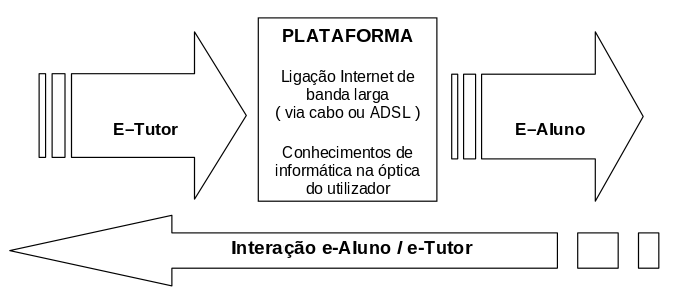
\includegraphics[keepaspectratio=true,scale=0.6]{figuras/e-learning-barbosa.png}
  \caption{Processo de \textit{e-Learning} por \citeonline{barbosa}}
  \label{fig:e-learning-caracterização-barbosa}
\end{figure}


É importante deixar claro que existem diferenças entre o \textit{e-Learning} e a EAD, enquanto a EAD é definido como qualquer ensino a distância, ou seja uma forma de educação em que o professor, conteúdo e aluno podem estar em locais e tempos diferentes, o \textit{e-Learning} é uma forma de Educação a distância que utiliza os meios tecnológicos como a Internet.


\subsubsection{AS VANTAGENS E DESVANTAGENS DO \textit{E-LEARNING}}
As principais vantagens do \textit{e-learning}, mostradas por \citeonline[p.~80]{hall} em seu artigo são: multiplicação dos pontos de treinamento, facilidade de acesso das informações, diminuição dos custos, remoção dos deslocamentos de funcionários, minimização do tempo usado em treinamentos, rapidez na atualização de conteúdos e definição do ritmo de aprendizagem pelo próprio aluno.
\citeonline[p.~5]{barbosa} aponta a flexibilidade e a disponibilização da informação em tempo real como uma vantagem importante do \textit{e-Learning}, assim o aluno consegue ter um tempo próprio para aulas, podendo acessar as aulas a qualquer hora e local.

Segundo \cite[p.~6]{bernardo} no \textit{e-learning}, o sistema computadorizado ou o treinador podem detectar mais facilmente falhas ou dificuldades dos alunos e corrigi-las imediatamente, de modo que isso não afete negativamente o aprendizado.

No entanto a alta robotização do treinamento pode gerar dificuldades tanto em alunos como em professores, por ser algo relativamente novo, não existem muitas pessoas com experiência para desenvolver aulas on-line. \cite[p.~6]{bernardo} aponta para o problema de que os alunos podem não se sentir à vontade para participar de aulas virtuais, porque acham muito importante o encontro físico entre alunos e professores na sala de aula.

A plataforma também deve ser simples de manusear, facilitando a interatividade e tendo o apoio do formador, para poder tirar dúvidas, partilhar informações e experiências. Se os alunos tiverem dificuldades em usar a tecnologia disponibilizada na plataforma, podem perder mais tempo para aprender a usar a plataforma, do que o acesso ao seu conteúdo. \apud[p.~5]{barbosa}{choi}

\citeonline[p.~6]{barbosa} aponta também uma controvérsia da \quotes{ausência} de relação humana, o que pode gerar ou não isolamento por parte do aluno. Mesmo que o aluno possa estar sozinho no local de acesso, ele poderá ter a companhia dos colegas virtuais e até do professor.

\subsubsection{E-LEARNING APOIADO POR VÍDEOS}
O vídeo se tornou um recurso de fácil acesso, mas seu uso na educação somente começou a partir da década de 90, \citeonline{moran} foi um dos pioneiros a escrever sobre esse assunto no Brasil com o artigo \quotes{O Vídeo na Sala de Aula}, no texto o autor fala sobre as linguagens da TV e do vídeo, e também sobre seu impacto na comunicação.

\citeonline[p.~3]{moran} destaca pontos importantes na utilização de vídeos na educação como: auxiliar o despertar da curiosidade, permite desenvolver cenários desconhecidos pelos alunos, proporciona simulações de realidade, reproduz também documentários, entrevistas, depoimentos e ajuda no desenvolvimento do senso crítico. Segundo \citeonline[p.~3]{moran}:
\begin{citacao}
  As tecnologias são pontes que abrem a sala de aula para o mundo, que representam, medeiam o nosso conhecimento do mundo. São diferentes formas de representação da realidade, de forma mais abstrata ou concreta, mais estática ou dinâmica, mais linear ou paralela, mas todas elas, combinadas, integradas, possibilitam uma melhor apreensão da realidade e o desenvolvimento de todas as potencialidades do educando, dos diferentes tipos de inteligência, habilidades de atitudes.
\end{citacao}

\section{SISTEMA DE GESTÃO DE APRENDIZADO (\textit{LMS})}
\label{sec:lms}

\citeonline[p.~2]{andrade} descreve o \ac{LMS} como um \textit{software} que controla o desenvolvimento, gerenciamento e acompanhamento de cursos de aprendizagem online. O \ac{LMS} é um sistema de gestão que possui funcionalidades para suportar o aprendizado a distância tais como: distribuição, acompanhamento, monitoramento e administração de conteúdo de aprendizagem com os progressos e interações dos alunos.
Segundo \citeonline[p.~3]{goni}:
\begin{citacao}
  Um \textit{LMS} tem como um dos objetivos, simplificar a administração dos programas de treinamento e ensino em uma organização. O sistema auxilia no planejamento dos processos de aprendizagem e ainda permite que os participantes colaborem entre si através da troca de informações e conhecimentos.
\end{citacao}

Esses sistemas ajudam na disponibilidade das informações, análises, rastreamento de dados e a geração de relatórios sobre o andamento dos cursos.

As principais funcionalidades do sistema \ac{LMS}, são:
\begin{itemize}
  \item Criar e administrar cursos;
  \item Oferecer ferramentas de comunicação como listas de discussão, \textit{chats} e mensagens instantâneas;
  \item Administrar grades curriculares e listagens de espera;
  \item Fornecer tarefas, avaliações e exercícios;
  \item Monitorar o acesso do usuário;
  \item Administrar matrículas de aprendizes;
  \item Gerar relatórios e informações sobre o desempenho dos aprendizes, etc;
\end{itemize}

\subsection{\textit{MOODLE}}
O \ac{Moodle} (Ambiente de Aprendizagem Dinâmico Modular Orientado a Objetos), é um software livre criado pelo australiano Martin Dougiamas no ano de 1999, é um software de gerenciamento de cursos que auxilia os professores a criarem cursos \textit{on-line}. Muito usado em cursos à distância por possuir funcionalidades que ajudam o professor no processo de avaliação além promover aprendizagem colaborativa. O \ac{Moodle} é um \textit{software} livre fornecido gratuitamente sobre a licença \textit{GNU Public License}\footnote{www.gnu.org/copyleft/gpl.html}. \cite{moodle}

O \ac{Moodle} foi criado para ser flexível e fácil de ser modificado. Foi escrito usando-se a linguagem \ac{PHP}, que o faz funcionar em qualquer plataforma de computador com um mínimo de esforço. Segundo o site oficial do Sistema, existem mais de 49 mil sites registrados com o sistema em 214 países \cite{moodle-stats}

O motivo da adoção do sistema por varias organizações é a sua facilidade de instalação e atualização, ser livre, apresentar grande flexibilidade nas configurações e oferecer recursos tecnológicos úteis para a EAD.

Uma das vantagens do \ac{Moodle} é a possibilidade do uso de padrões abertos como o \ac{SCORM} e o \ac{LTI} o que o torna uma plataforma é interoperável, permitindo a integração de aplicações externas e informações em uma única plataforma \ac{Moodle}.

A plataforma é divida em blocos e módulos, como a maioria dos portais \textit{Web} conhecidos como \ac{CMS}. No entanto o \ac{Moodle} é categorizado como um \ac{LMS}. Utilizando essa arquitetura, novos módulos podem ser desenvolvidos de forma independente, e disponibilizados e utilizados de acordo com a necessidade.

\subsection{Padrões de \textit{E-Learning}}
Segundo a ISO, padrões são definidos como \quotes{acordos documentados que contém especificações técnicas ou outros critérios precisos que são usados como regras, guias ou definições de características de modo a garantir que materiais , produtos, processos e serviços sirvam a seus propósitos}.

Com o crescimento do uso do computador pessoal as tecnologias digitais vem aumentado na área da educação, porem, essas tecnologias são desenvolvidas em formas divergentes, diversos cursos, módulos e sistemas desenvolvidos para fornecer os cursos, são criados independentemente um dos outros, geralmente isso gera mais custos e esforço, por que sem o uso de um padrão, um curso precisa ser desenvolvido diversas vezes para funcionar em vários \ac{LMS}.

Sem uma especificação de como os cursos devem ser feitos, os desenvolvedores da ferramenta, geralmente esperam que outros se conformem com sua própria estrutura dificultando assim a interoperabilidade entre os sistemas.

Segundo \citeonline[p.~8]{bianco-standards}, existem quatro vantagens no desenvolvimento de cursos e ferramentas usando um padrão do \textit{e-learning}, são esses:
\begin{itemize}
  \item Durabilidade: Não é necessário realizar modificações na integração se a versão do \textit{software} mudar.
  \item Interoperabilidade: Funcionamento em uma grande variedade de sistemas para qual o padrão foi desenvolvido, como é o caso dos \textit{LMS}.
  \item Acessibilidade: Indexação e rastreamento sob demanda do conteúdo.
  \item Reusabilidade: Possibilidade de uso em diversas outras ferramentas.
\end{itemize}

Para esse projeto, foram analisados dois dos mais conhecidos padrões de \textit{e-learning}, e escolhido o mais adequado para o caso de uso, os padrões \ac{SCORM} e o \ac{LTI}.

\subsubsection{\textit{SCORM (Shareable Content Object Reference Model)}}
O \ac{SCORM} teve a sua primeira versão lançada em 2000, pela \ac{ADL}, um consórcio de grupos internacionais em tecnologias educativas, liderado pelo Departamento de Defesa dos Estados Unidos, visando a pesquisa e criação de recursos para aprendizagem \cite{adl}.

Segundo \citeonline[p.~24]{fernandes-scorm}, uma das grandes características do \ac{SCORM} é sua reutilização e interoperabilidade, dando independência da plataforma onde os objetos do SCORM podem ser usados, facilitando assim a migração dos cursos entre os diferentes \ac{LMS} compatíveis com esse modelo. O \ac{SCORM} é um conjunto de especificações para a disponibilização de conteúdos e serviços de aprendizagem pelo computador e a \ac{WEB} \cite{adl}.

A especificação do \ac{SCORM} está dividido em 4 documentos, chamados de livros pela \cite{adl}, são eles:
\begin{enumerate}
  \item \textbf{\textit{The Scorm Overview}}: Descreve o \ac{SCORM} em geral, definindo seus conceitos sobre o modelo.
  \item \textbf{\textit{The SCORM content Aggregation Model (CAM)}}: Descreve os componentes usados em uma interação de aprendizagem, mostrando como empacotar os cursos e realizar a migração entre os ambientes de aprendizagem, descreve também os metadados que precisam ser usados na descrição do objeto de aprendizagem.
  \item \textbf{\textit{The SCORM Run-Time Enviroment (RTE)}}: Trata da execução dos objetos criados no modelo \ac{SCORM}, por exemplo, como é feita a comunicação do objeto com o ambiente de aprendizagem.
  \item \textbf{\textit{The SCORM Sequencing and Navigation (SN)}}: Trata do navegação do conteúdo do objeto de aprendizagem, descrevendo como deve ser feita a navegação através do conteúdo do objeto construído.
\end{enumerate}

\begin{figure}[h]
  \centering
  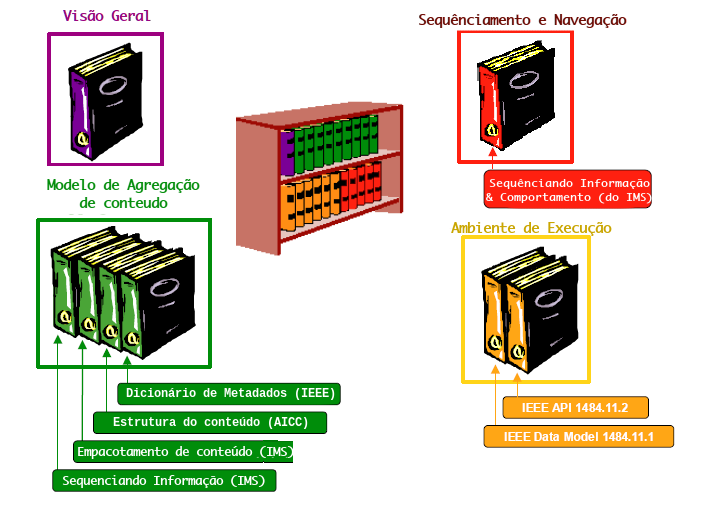
\includegraphics[keepaspectratio=true,scale=0.7]{figuras/scorm-funcionamento-dutra_traduzido.png}
  \caption{SCORM como conjunto de especificações. Fonte: \citeonline[tradução nossa]{dutra-scorm-ims}}
  \label{fig:scorm-funcionamento-dutra}
\end{figure}

O pacote \ac{SCORM} gerado tem como resultado um arquivo \textit{ZIP}, esse arquivo contem o conteúdo do curso, e também deve possuir todos os arquivos \textit{HTML}, \textit{Javascript}, imagens e animações, além de um arquivo de manifesto chamado \textit{imsmanifest.xml}. Este arquivo descreve a estrutura lógica do conteúdo como a navegação das páginas e a organização de todo conteúdo. O \ac{LMS} carrega esse pacote e então cria o relacionamento entre as unidades (Pacote \textit{SCORM} e o \textit{LMS}). \cite[p.~39]{fernandes-scorm}.

Como o \textit{SCORM} e distribuído como um pacote \textit{ZIP}, permite que os seus conteúdos resistam a evolução tecnológica, com custo baixo de reconfiguração, esse pacote pode ser reaproveitado em \textit{LMS} compatíveis com seu funcionamento inalterado.

Mesmo sendo o padrão \textit{e-learning} mais famoso, o \textit{SCORM} é um padrão antigo e está ficando ultrapassado por alguns problemas que ele apresenta. Um dos problemas é a falta de segurança, o padrão necessita que os dados do aluno fiquem salvos no navegador do próprio, geralmente no \textit{cache} do navegador, incluindo as respostas da atividade, dessa forma um aluno com o conhecimento dessa falha pode verificar os dados salvos pela atividade.

Outro problema é o fato de que todo o curso fica em um pacote \textit{zip}, e para reutilizar é necessário duplicar esse pacote, isso pode resultar em uma carga no disco onde o \textit{LMS} está hospedado.

\subsubsection{\textit{LTI (Learning Tool Interoperability)}}
\label{sec:lti}

O \textit{LTI} foi criado pela \textit{IMS}, a primeira versão TI 1.0 foi lançado em 2006 mais na época foi considerado muito complexo, e não teve uma boa adoção. O projeto do \textit{Learning Tools Interoperability} foi desenvolvido com os mesmos objetivos do TI, mais com uma solução mais simples. \cite{ims}

A versão atual do \textit{LTI} é a 1.1, que suporta dados de retorno ao \textit{LMS} como as notas que ao aluno atingiu no curso.

\begin{citacao}
  O \textit{LTI} tem a habilidade de fornecer á um usuário em um \textit{LMS} (Ou outro sistema \textit{web} com suporte ao padrão) de acessar uma aplicação de aprendizagem separada, um item de conteúdo protegido ou outro recurso restrito. \cite[p.~2, tradução nossa]{vickers-ims}
\end{citacao}

Quando um usuário que está em um \textit{LMS} para um sistema com suporte ao \textit{LTI} alguns dados são enviados juntos a ele:
\begin{itemize}
    \item Detalhes sobre ele (como nome e email);
    \item Detalhes sobre o contexto institucional (como o nome do \textit{LMS que está sendo usado, nome da faculdade});
    \item Detalhes do contexto de onde o usuário está vindo (como o curso especificado);
    \item A sua função no \textit{LMS} (como professor ou aluno);
\end{itemize}
Esses dados são fornecidos pelo próprio \textit{LMS}, no seu lançamento.

O lançamento do sistema externo ocorre de maneira segura (usando \textit{OAuth}) pelo navegador do usuário. Uma conexão é criada entre esses dois sistemas por meio de autenticação, as únicas informações que o \textit{LMS} precisa sobre o sistema externo são:
\begin{itemize}
    \item A \ac{URL} do sistema;
    \item Uma chave para identificar o cliente (chamada de \textit{\quotes{consumer key}} ou chave do cliente);
    \item Uma outra chave secreta para proteger a conexão(chamada de \textit{shared secret});
\end{itemize}

Segundo \citeonline[p.~2]{vickers-ims} o sistema de Gestão de Aprendizagem (\textit{LMS}), na especificação do \textit{LTI}, é chamado de \ac{TC} em português seria algo como \quotes{Consumidor da Ferramenta}, que é o sistema que irá \quotes{consumir} a outra aplicação ou recurso, que é provido pelo \ac{TP} em português \quotes{Provedor da Ferramenta}.

Um \textit{TP} pode ser tanto um \textit{LMS} como um portal empresarial, ou qualquer sistema que suporte a implementação do \textit{LTI}. É um \textit{TC}, pode ser um \textit{Wiki} (Um site de edição coletiva) ou uma ferramenta de questionários por exemplo.
\begin{figure}[h]
    \centering
    \label{fig:ims-lti-funcionamento}
    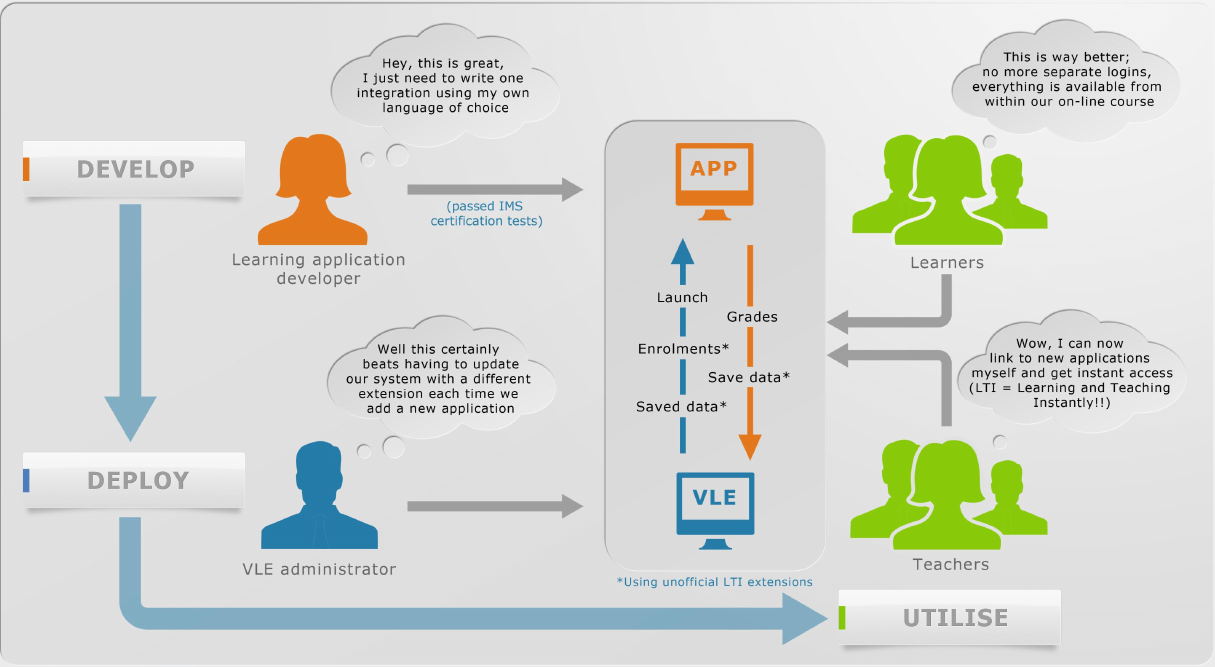
\includegraphics[keepaspectratio=true,scale=0.5]{figuras/ims-lti-funcionamento.png}
    \caption{Funcionamento do \textit{LTI}. Fonte: \citeonline{ims}}
\end{figure}

Quando um usuário clica em um link referente à um \textit{TP}, a plataforma de aprendizagem envia junto com os dados um assinatura \textit{OAuth}. \textit{OAuth} é um protocolo aberto que permite a autorização segura em um método simples e padronizado em aplicações \textit{web}, \textit{desktop} e móveis, \cite{oauth}, permitindo que o \textit{TP} confie que a informação na requisição de lançamento é de um \textit{TC}.

Quando \textit{tool provider} recebe a requisição, ele então usa a chave \textit{shared secret} para decifrar a informação e assegurar que a requisição é de um \textit{LMS}. O \textit{tool provider} usa também outras informações na requisição para mostrar a aplicação com as configurações corretas para o usuário e seu contexto (como uma ligação entre o curso e a aplicação).

Uma requisição de lançamento LTI (\textit{LTI launch}) é um \textit{POST} \ac{HTTP} enviado pela plataforma de aprendizagem com uma \textit{array} de elementos escondidos do form (\textit{hidden form elements}). Quando o \textit{TP} recebe a requisição, ele valida a informação, cria a conta de usuário (se necessário) e a ligação com o curso, e então cria uma sessão e redireciona o navegador do usuário para a página da ferramenta.

\chapter{TECNOLOGIAS UTILIZADAS NO SISTEMA}

Para que a Ferramenta fosse desenvolvida, foi realizado um estudo das ferramentas que melhor atenderiam esse processo. A escolha foi baseada principalmente priorizando as tecnologias que já se tinha conhecimento, e também na facilidade de uso.

\section{PADRÕES ARQUITETURAIS}
Nessa seção apresentarei os dois padrões arquiteturais que foram usados nesse projeto, o \ac{MVC} e o \ac{MVVM}.

\subsection{\textit{MVC (Model-View-Controller)}}
\label{sec:mvc}

    \begin{figure}[h]
        \centering
        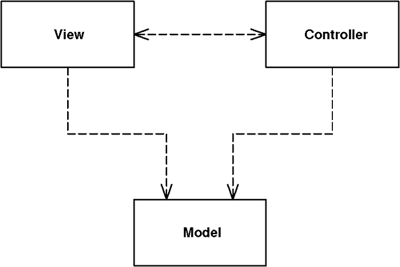
\includegraphics[keepaspectratio=true,scale=0.7]{figuras/mvc-fowler.png}
        \caption{Ilustração do \ac{MVC}, fonte: \cite{martin_fowler_patterns}}
        \label{fig:mvc-fowler}
    \end{figure}

\textit{Model View Controller (MVC)}, começou como um \textit{framework} criado por Trygve Reenskaug para a plataforma Smalltalk em 1970. \cite[p.~321]{martin_fowler_patterns}.

Segundo \citeonline[p.~321]{martin_fowler_patterns} o \ac{MVC} consiste em três regras, descritas na tabela~\ref{tbl:mvc}:

\begin{table}[htp]
    \begin{center}
        \begin{tabular}{|l|p{10cm}|}
            \hline \textbf{Regra} & \textbf{Descrição} \\
            \hline \textit{Model} (Modelo) & 
            O \textit{model} é um objeto que representa informações sobre o domínio. É um objeto não visual, que contem todos os dados e comportamentos, diferente do utilizado para a UI. \\
            \hline \textit{View} (Apresentação) & 
            A \textit{view} representa a visualização do \textit{model} na \ac{UI} \\
            \hline \textit{Controller} (Controle) & 
            O \textit{controller} tem o papel de receber entradas do usuário, manipular o \textit{model}, e atualizar a \textit{view}. \\
            \hline
        \end{tabular}
        \caption{Descrição do \ac{MVC}.}
        \label{tbl:mvc}
    \end{center}
\end{table}

Um dos pontos principais na separação do \ac{MVC} é a direção das dependências, a camada da apresentação (\textit{view}) depende do \textit{model}, mais o \textit{model} não depende da \textit{view}, por causa dessa separação, quem estiver desenvolvendo o \textit{model} não precisa saber como a apresentação está sendo feita, facilitando que a criação das apresentações. Isso significa também que as mudanças na apresentação podem ser feitas livremente sem afetar o modelo.

\citeonline[p.~322]{martin_fowler_patterns}, também cita alguns pontos importantes dessa separação, como o fato de que quando está desenvolvendo uma apresentação, é necessário se concentrar na \ac{UI} e como criar uma boa interface. E quando se está construindo um modelo é necessário pensar nas politicas comerciais também nas interações com o banco de dados. Testes também se tornam mais simples com essa separação, porque objetos não visuais são mais fáceis de testar do que os visuais, separando a apresentação do \textit{model}, permite que seja feito testes na logica do domínio facilmente sem se importar com a \ac{UI} do sistema.
\subsection{\textit{MVVM (Model-View-ViewModel)}}
\label{sec:mvvm}

    \begin{figure}[h]
        \centering
        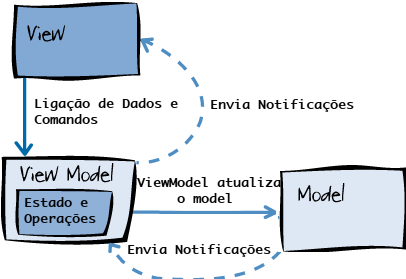
\includegraphics[keepaspectratio=true,scale=0.8]{figuras/mvvm-microsoft-traduzido.png}
        \caption{Ilustração do funcionamento do \textit{MVVM}, fonte: \cite[tradução nossa]{ms_mvvm}}
        \label{fig:mvvm-microsoft}
    \end{figure}

O \ac{MVVM} é um padrão que foi criado em 2005 por John Gossman, um dos arquitetos do \ac{WPF}\footnote{Windows Presentation Foundation (WPF) no Visual Studio de 2015 fornece aos desenvolvedores um modelo de programação unificado para criar aplicativos de área de trabalho de linha de negócios modernos no Windows. \url{https://msdn.microsoft.com/pt-br/library/aa970268\%28v=vs.110\%29.aspx}} e \textit{Silverlight} na \textit{Microsoft}.

Segundo a \citeonline{ms_mvvm}, o \acf{MVVM} foi criado para realizar uma separação clara entre a interface do usuário e a logica. o padrão \ac{MVVM} é composto por três componentes: O \textit{model} (Modelo), a \textit{view} (Apresentação) e a \textit{ViewModel}, cada um tem um papel distinto, a ilustração~\ref{fig:mvvm-microsoft} mostra a relação entre os três componentes, como mostrado na tabela~\ref{tbl:mvvm}.

\begin{table}[htp]
    \begin{center}
        \begin{tabular}{|l|p{11cm}|}
            \hline \textbf{Componente} & \textbf{Descrição} \\
            \hline \textit{View} (Apresentação) & 
            A camada de apresentação, é responsável por definir a estrutura, \textit{layout} e aparência do que o usuário vê na tela.
            
            Uma apresentação por ter seu próprio \textit{view model}. ou pode herdar do \textit{view model} principal. A \textit{view} recebe os dados do seu \textit{view model} por meio de \textit{bindings} (ligações), ou invocando métodos no \textit{view model}. Em tempo de execução, a \textit{view} se modifica quando os controles da interface do usuário (UI) responde  as propriedades do \textit{view model} quando ele dispara eventos de modificação.
             \\
            \hline \textit{Model} (Modelo) & 
            O modelo na \textit{MVVM} é uma implementação do modelo de domínio da aplicação, que inclui um modelo de dados, juntamente com a lógica de negócio e validação. \\
            \hline \textit{View Model} & 
            O \textit{view model} é uma camada intermediaria entre a \textit{view} e o \textit{model}, e tem a responsabilidade de tratar a lógica da camada de apresentação. A camada \textit{view model} interage com o \textit{model} chamando métodos no \textit{model}, então o \textit{view model} envia os dados recebidos do \textit{model} de uma forma que a \textit{view} possa utilizar de forma simples, com a possibilidade de formatar esses dados para facilitar seu uso na \textit{view}. \\
            \hline
        \end{tabular}
        \caption{Descrição do \ac{MVVM}.}
        \label{tbl:mvvm}
    \end{center}
\end{table}

\begin{citacao}
    O MVVM permite a você ter uma visão da clara separação da Interface com o usuário (View), sua lógica de apresentação (ViewModel) e os seus Dados (Model). E, trabalhando dessa forma, temos separação de responsabilidades, desacoplamento e conseguimos evoluir e manter melhor as nossas aplicações. \cite{ferreira_mvvm}
\end{citacao}

Como é mostrado na figura~\ref{fig:mvvm-microsoft} e também descrito por \citeonline{ferreira_mvvm}, o processo do \textit{MVVM} ocorre dessa forma: A \textit{View}, através do \textit{databinding}, interage com a \textit{ViewModel} notificando algum evento. A \textit{ViewModel} responde a essa notificação, realizando alguma ação no modelo, como obter algum dado, atualizar ou inserir informações. Caso alguma informação seja modificado no \textit{Model}, a \textit{ViewModel} recebe uma notificação de atualização, que em seguida, notifica também a \textit{view} com essa atualização.

\section{PHP}
\label{sec:php}

Atualmente a abreviação \textit{PHP} vem de \textit{Hypertext Preprocessor}, é uma linguagem de programação de código aberto muito usada para \textit{scripts} que são usados juntamente a um servidor web para servir páginas \textit{HTML}.

A linguagem de programação PHP foi criada em 1994 por Rasmus Lerdorf, no inicio era formada por um conjunto de \textit{scripts} voltados à criação de páginas dinâmicas, em que Rasmus usava para monitorar o acesso ao seu currículo na internet, mais a medida que a ferramenta foi crescendo em suas funcionalidades, Rasmus teve de escrever uma implementação em C, permitindo que as pessoas desenvolvessem de forma mais simples suas aplicações web, e então a chamou de PHP/FI (\textit{Personal Home Pages/Forms Interpreter}) e disponibilizou seu código em 1995 neste momento o \textit{PHP} começou a ser um projeto comunitário desenvolvido por uma equipe de colaboradores. \cite[p.~20]{pablo-php}.

\begin{listing}
    \begin{phpcode}
    <!DOCTYPE HTML PUBLIC "-//W3C//DTD HTML 4.01 Transitional//EN"
    "http://www.w3.org/TR/html4/loose.dtd">
    <html>
        <head>
            <title>Exemplo</title>
        </head>
        <body>

        <?php
            echo "Olá, eu sou um script PHP!";
        ?>

        </body>
    </html>
    \end{phpcode}
    \caption{Código simples de PHP retirado do site http//php.net:}
    \label{lst:php_example_1}
\end{listing}

Os paginas \textit{PHP} contém \textit{HTML} com código embutido executando alguma ação como no exemplo acima \ref{lst:php_example_1}, o resultado será \quotes{Olá, eu sou um script PHP!}.

O código \textit{PHP} é delimitado pelas instruções de processamento (\textit{tags}) de início e fim \textit{<?php e ?>} que permitem que você escreva o código dentro e fora do \textit{PHP} no mesmo arquivo \textit{HTML}. \cite{php-intro}

O \textit{PHP} é executado no lado do servidor (server-side), gerando um \textit{HTML} que é enviado para o cliente que recebe os resultados da execução desse \textit{script}, mais não tem acesso ao seu código fonte. Na página do Manual do \textit{PHP} diz o seguinte: \quotes{A melhor coisa em usar o PHP é que ele é extremamente simples para um iniciante, mais oferece muitos recursos para um programador profissional} \citeidem{php-intro}. A simplicidade do \textit{PHP} é uma das suas melhores qualidades que a mantêm entre as 3 linguagens mais usadas como mostra o infográfico da \citeonline{iinterativa}.

O \textit{PHP} também pode ser utilizado na maioria dos sistemas operacionais, incluindo \textit{Linux}, \textit{Solaris}, \textit{OpenBSD}, \textit{Microsoft Windows}, Mac OS X. Também é suportado pela maioria dos servidores web atualmente, como o \textit{Apache}, \textit{IIS}, \textit{Nginx} e \textit{lighttpd}, dando assim uma liberdade de escolha do sistema operacional e do servidor web. O \textit{PHP} também oferece suporte para uma ampla variedade de banco de dados\footnote{Extensões de Banco de Dados \url{http://php.net/manual/pt_BR/refs.database.php}}.


\section{APACHE}
\label{sec:apache}

Um servidor \textit{WEB} é responsável de aceitar requisições \textit{HTTP} dos clientes \textit{web} e servi-los com respostas \textit{HTTP} geralmente na forma de paginas com conteúdo estático como texto e imagens, e conteúdos dinâmicos como \textit{scripts} \cite[p.~15]{igor}.

Em 1995 Robert McCool desenvolvedor da \ac{NCSA} criou um servidor \textit{Web} chamado \textit{NCSA HTTPd} que se tornou o mais utilizado na época, por problemas de comunicação e gerenciamento dos \textit{patchs} do servidor, foi então criado o \textit{Apache Group}, que usou o código do \textit{NCSA Web Server} e criou um novo servidor chamado \textit{Apache}. \cite[p.~36]{kabir}.

A importância principal do \textit{Apache} para o projeto, é o seu suporte completo ao \textit{PHP}. O \textit{Apache} também é um servidor simples e totalmente configurável por meio de um arquivo,  chamado \textit{httpd.conf} que pode ser aberto em qualquer editor de texto, outros fatores importantes descritos por \cite[p.~38]{kabir}, que são relevantes para o projeto são:
\begin{itemize}
    \item Suporte ao protocolo HTTP 1.1 e atualmente suporte ao novo HTTP 2, por meio de um modulo chamado mod\_h2 \footnote{\url{https://github.com/icing/mod_h2}}.
    \item Suporte a \textit{Virtual Host} que é a capacidade de hospedar mais do que um site em uma única máquina.
    \item Suporte a \textit{.htaccess} que são arquivos que permitem realizar mudanças nas configurações por diretórios, sem precisar editar o \textit{httpd.conf} novamente.
\end{itemize}

O \textit{Apache} é também o servidor \textit{web} mais utilizado no mundo, segundo a pesquisa do \citeonline{netcraft-survey} mostrado na tabela \ref{tbl:netcraft}.

\begin{table}[htp]
    \tiny
    \centering
    \begin{tabular}{|>{\centering\arraybackslash} p{.17\textwidth}| >{\centering\arraybackslash} p{.16\textwidth}|>{\centering\arraybackslash} p{.12\textwidth}| >{\centering\arraybackslash} p{.16\textwidth}|>{\centering\arraybackslash} p{.12\textwidth}|>{\centering\arraybackslash} p{.11\textwidth}|}
        \hline \textbf{Desenvolvedor} & \textbf{Julho 2015} & \textbf{Pct \%} & \textbf{Agosto 2015} & \textbf{Pct \%} & \textbf{Mudança} \\
        \hline Apache                 & 325,696,514         & 38.34\%         & 327,985,968          & 37.51\%         & -0.83            \\
        \hline Microsoft              & 225,282,713         & 26.52\%         & 231,429,146          & 26.47\%         & -0.05            \\
        \hline nginx                  & 131,460,063         & 15.47\%         & 132,443,391          & 15.15\%         & -0.33            \\
        \hline Google                 & 20,255,424          & 2.38\%          & 19,933,095           & 2.28\%          & -0.10            \\
        \hline
    \end{tabular}
    \centering
    \caption{Tabela com as estatísticas de uso dos servidores web pela netcraft em Agosto de 2015}.
    \label{tbl:netcraft}
\end{table}

\section{MYSQL}
\label{sec:mysql}

Segundo \citeonline[p.~38]{mysql-reference}, O \textit{MySQL} é um sistema de gerenciamento de banco de dados relacional \textit{SQL Open Source}, desenvolvido pela \textit{MySQL AB} uma empresa Sueca fundada por David Axmark, Allan Larsson e Michael Widenius.

Em janeiro de 2008, a empresa \textit{MySQL AB}, foi adquirida pela \textit{Sun Microsystems}, por US\$ 1 bilhão\footnote{\url{http://www.zdnet.com/article/sun-acquires--adds-to-its-software-stack/}}. E em abril de 2009 a \textit{Oracle} comprou a \textit{Sun Microsystems} e todos os seus produtos\footnote{\url{http://www.oracle.com/us/corporate/press/018363}}.

Assim como o \textit{PHP}, o \textit{MySQL} é um \textit{software} de código aberto, possuindo dois tipos de licença: a licença para uso Livre \ac{GPL}, sem custos, e a licença comercial, necessária para usar o \textit{MySQL} em aplicações comerciais.

\citeonline[p.~38]{kofler} e \citeonline[p.~40]{mysql-reference} lista algumas das características relevantes do \textit{MySQL}, as quais são:
\begin{itemize}
    \item \textbf{Compatibilidade com SQL}: O \textit{MySQL} suporta a linguagem \textit{SQL (Strutured Query Language)}, \textit{SQL} é uma linguagem padrão para consultas e atualização de dados em um banco de dados.
    \item \textbf{Independência de Plataforma}: O Servidor do \textit{MySQL} pode ser executado na maioria dos sistemas operacionais, os mais importantes são: \textit{Microsoft Windows}, \textit{Linux}, \textit{Apple Macintosh OS X} e as variantes do \textit{UNIX}.
    \item \textbf{Compatibilidade}: Existem muitas \textit{APIs} e bibliotecas para o \textit{MySQL} que permitem que ele se comunique com diversas linguagens de programação como: \textit{PHP, C/C++, Java, C\#, Python, Perl} entre outras.
    \item \textbf{Segurança}: A segurança do \textit{MySQL} é feito por um sistema de privilégios e senhas flexíveis, seguro e que permite a verificação baseada em estações/máquinas. Todo o tráfico de senhas é criptografado quando você se conecta ao servidor.
    \item \textbf{Estabilidade}: Consegue lidar com bancos de dados enormes. Com capacidade de armazenação e manipulação de tabelas com mais de 50.000.000 registros.
\end{itemize}



\section{\textit{FRAMEWORKS} E BIBLIOTECAS}

\subsection{\textit{LARAVEL}}
\label{sec:laravel}

O \textit{Laravel} é um \textit{framework PHP} de código aberto, criado por Taylor Otwell, para o desenvolvimento de aplicações \textit{WEB}, seguindo o padrão arquitetural \ac{MVC}.
Código aberto, criado por Taylor Otwell para o desenvolvimento

O motivo da escolha do \textit{framework laravel} para o projeto, são algumas características que simplificam o desenvolvimento, e permitem uma melhor modularizarão do código, como por exemplo essas listadas por \citeonline[p.~24]{bean-laravel}:
\begin{itemize}
  \item \textbf{Roteamento}: O \textit{Laravel} fornece muita flexilidade na definição de rotas da aplicação. É possível por exemplo, ligar todas as ações do \textit{controller} para suas rotas, como na rota \quotes{cursos/create} (\textit{CursosController}, ação \textit{create}), ou criar rotas de \ac{REST} que são principios que definem como rotas HTTP devem ser usadas, o padrão facilita também o uso das rotas como API para usa-las em outras aplicações. As rotas \textit{REST} são: \textit{GET}, \textit{POST}, \textit{PUT} ou \textit{DELETE}.

  \item \textbf{\textit{Query Builder} e \ac{ORM}}: O \textit{framework} também fornece um \textit{query builder} (construtor de consultas) chamado de \textit{Eloquent}, que permite criar consultas do banco de dados utilizando a \textit{syntax} do \textit{PHP}, permitindo um agrupamento de métodos em vez de escrever \ac{SQL}.

  Por exemplo, a seguinte consulta do \textit{SQL}:
  \begin{listing}
    \begin{sqlcode}
      SELECT * FROM cursos c where user_id = 1
      JOIN m markers as m.curso_id = c.id
      ORDER BY c.created_at
      LIMIT 10
    \end{sqlcode}
    \caption{Busca simples do SQL. Buscar todos os cursos em que o user\_id seja igual a 1, unir os resultados com a tabela markers, ordenar pela data de criação do curso, e limitar os resultados por 10}
    \label{lst:sql_example_eloquent}
  \end{listing}

  Pode ser escrita dessa forma usando o \textit{Eloquent}:
  \begin{listing}
    \begin{phpcode}
      <?php
      App\Curso::with("markers") // Buscar da tabela cursos com a tabela markers
      ->where("user_id", 1) // Somente se o user_id == 1
      ->orderBy("created_at") // Ordenar pela data de criação dos cursos
      ->take(10) // Limitar os resultados por 10
      ->get(); // Executar a consulta
      ?>
    \end{phpcode}
    \caption{Consulta \ref{lst:sql_example_eloquent} em Eloquent}
    \label{lst:php_example_eloquent}
  \end{listing}

  \item \textbf{Sistema de \textit{Templates}}: O \textit{Laravel} fornece um sistema de \textit{template} chamado de \textit{Blade}, que permite a criação de \textit{layouts} hierárquicos.
\end{itemize}

\subsection{JQUERY}
\label{sec:jquery}

\begin{citacao}
    jQuery é uma biblioteca de Javascript, rápida, pequena e rica em recursos. Ela faz com que coisas como seleção e manipulação do HTML, manipulação de eventos, animações e Ajax muito mais simples, com uma API fácil de usar que funciona em uma vasta quantidade de navegadores. Com uma combinação de versatilidade e capacidade de extensão, o jQuery mudou a maneira de milhões de pessoas que escrevem JavaScript. \cite[tradução nossa]{jquery}
\end{citacao}

O \textit{jQuery} é uma biblioteca \textit{JavaScript} criada por Jogn Resig e disponibilizada como software livre e aberto, utilizando a licença \ac{MIT}\footnote{\url{https://tldrlegal.com/license/mit-license}}, o que significa que pode-se usar a biblioteca gratuitamente em projetos pessoais como comerciais.

Segundo \cite[p.~4]{silva-jquery}, o \textit{jQuery}, se destina a adicionar interatividade e dinamismo às paginas web, incrementando a usabilidade, acessibilidade e o design da pagina, enriquecendo assim a experiência do usuário. \citeidem{silva-jquery}, diz também que a biblioteca pode ser usada para:
\begin{itemize}
    \item Adicionar efeitos visuais e animações;
    \item Acessar e manipular o DOM;
    \item Buscar informações no servidor sem a necessidade de recarregar a página (Ajax);
    \item Prover interatividade;
    \item Alterar conteúdos;
    \item Modificar apresentação e estilização;
    \item Simplificar tarefas especificas do \textit{JavaScript};
\end{itemize}

Uma das funcionalidades mais importantes do \textit{jQuery} é a possibilidade de acessar elementos do \ac{DOM}, que é uma plataforma que representa como as marcações em \textit{HTML, XHTML e XML} são organizadas e lidas pelo navegador \cite{franklin-dom}, utilizando seletores do \ac{CSS} para realizar a manipulação, diferente do código comum do \textit{JavaScript} em que o código e adicionado diretamente no elemento \textit{HTML} para definir qual elemento irá ser manipulado. como mostram os exemplos abaixo \ref{lst:javascript_example_1} e \ref{lst:jquery_example_1}.

\begin{listing}[htpb]
  \htmlfile{codigos/javascript_example_1.html}
    \caption{Código simples, mudando a cor e texto de um elemento usando \textit{javascript} puro.}
    \label{lst:javascript_example_1}
\end{listing}

Por usar chamadas nativas do \textit{Javascript} é possível que o código~\ref{lst:javascript_example_1}, não funcione corretamente em todos os navegadores. O código~\ref{lst:jquery_example_1} mostra um exemplo do código~\ref{lst:javascript_example_1} implementado em \textit{jQuery}.

Dessa forma se torna muito mais simples a manipulação de elementos do \textit{DOM} utilizando o \textit{jQuery}, outra característica que torna o \textit{jQuery} útil para esse projeto, é sua extensibilidade, por esse motivo, existem milhares de \textit{plugins} para \textit{jQuery} para diversas funcionalidades, inclusive o \textit{Video.JS}, a biblioteca utilizada para renderizar os vídeos, foi criada como um \textit{plugin} do \textit{jQuery}.

\begin{listing}[H]
    \htmlfile{codigos/jquery_example_1.html}
    \caption{Mudando a cor e texto de um elemento usando \textit{jQuery}}
    \label{lst:jquery_example_1}
\end{listing}

\subsection{VUE.JS}
\label{sec:vuejs}

No seu Site oficial \citeonline{vuejs}, O \textit{Vue.js} é descrito como uma biblioteca para criar interfaces web moderna, fornecendo componentes reativos com uma \textit{API} simples e flexiva.

\textit{Vue} é uma biblioteca criada utilizando o padrão \ac{MVVM}, que conecta a camada de \textit{View} com a de \textit{Model} usando \textit{two way data bindings}, as manipulações do \textit{DOM} feitas com essa biblioteca são abstraídas por meio de diretrizes e filtros.

Criada para ser uma biblioteca simples, com o intuito de realizar a separação de uma aplicação por meio de componentes. Diferente de \textit{frameworks MVC javascript} como o \textit{AngularJS, EmberJS ou Backbone}, o \textit{Vue} foi desenvolvida para utilizar somente a camada \textit{View} do \textit{MVC}.

Algumas das Funcionalidades importantes do \textit{Vue} são mostradas nas seções abaixo:

\subsubsection{Componentes}
\begin{figure}[h]
    \centering
    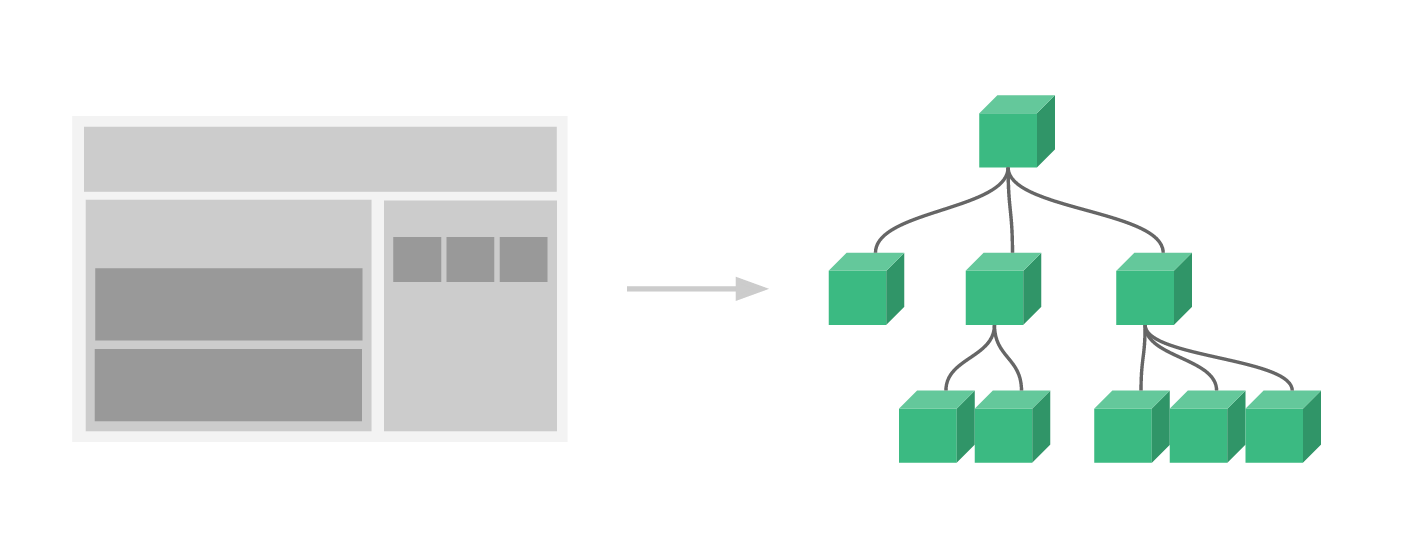
\includegraphics[keepaspectratio=true,scale=0.25]{figuras/vue-components.png}
    \caption{Ilustração dos componentes do \textit{Vue}, fonte: \cite{vuejs}}
    \label{fig:vue-components}
\end{figure}

No \textit{Vue.js}, cada componente é uma instancia do \textit{Vue}. Os componentes formam uma hierarquia de arvore aninhada que representa a interface da aplicação. Cada componente representa um elemento em uma aplicação (como um campo de texto, uma galeria ou um painel de notícias), os elementos estão ilustrados na figura~\ref{fig:vue-components} como os cubos verdes interligados.

Um componente deve ser desenvolvido com funcionamento padronizado, possibilitando o reuso em outras partes da aplicação.

\subsubsection{Diretrizes}
No \textit{Vue} as Diretrizes são atributos \textit{HTML} prefixados que dizem ao \textit{Vue.js} para fazer algo com o elemento \textit{DOM}.

\begin{listing}[H]
    \htmlfile{codigos/vue-directive.html}
    \caption{Exemplo de diretriz do \textit{Vue}}
    \label{lst:vue-directive-example}
\end{listing}

No exemplo~\ref{lst:vue-directive-example}, o elemento tem uma diretriz \textit{v-text} com o valor \quotes{texto}. Esse exemplo vai dizer ao \textit{Vue.js} para manter o conteúdo de texto da \textit{div} em sincronização com a propriedade \quotes{texto} da instância do \textit{Vue}. Dessa forma sempre que o valor do atributo for modificado, o conteudo da \textit{div} também será atualizado.

\subsubsection{Filtros}
Filtros são funções que processam o valor bruto de uma propriedade antes de atualizar a \textit{View}.
    \begin{listing}[H]
        \htmlfile{codigos/vue-filter.html}
        \caption{Exemplo de Filtro do \textit{Vue}}
        \label{lst:vue-filter-example}
    \end{listing}
    No exemplo~\ref{lst:vue-filter-example}, tudo que está dentro das chaves duplas será tratado pelo \textit{Vue} como uma expressão, no exemplo, o conteúdo da \textit{div} será atualizado de acordo com a mudança do atributo \textit{texto}. Mas antes do texto da \textit{div} ser atualizado, primeiro ele vai ser filtrado pela função \textit{uppercase} que por padrão coloca todo o texto em caixa alta. A função \textit{uppercase} e vem por padrão no \textit{vue} mas os filtros podem ser criados de forma customizada na instancia do \textit{vue}.

\subsection{BROWSERIFY}
\label{sec:browserify}

O \textit{Browserify} é uma ferramenta desenvolvida com \textit{javascript} que permite usar a função \textit{require} do \textit{NodeJS} (Interpretador \textit{javascript} do lado do servidor) diretamente no navegador, empacotando todas as dependências do seu projeto em um ou poucos arquivos \cite{browserify}.

O \textit{Browserify} permite que você escreva seu código \textit{javascript} e somente use as bibliotecas necessárias para determinado modulo, por meio da função \textit{require(./nome\_do\_\\arquivo.js)}, o \textit{browserify} também funciona com o \ac{NPM}, que é um gerenciador de pacotes do \textit{NodeJS} e de bibliotecas/\textit{frameworks} \textit{javascript} em geral. Isso permite que você instale a biblioteca \textit{Vue} por exemplo, usando \textit{npm} e a use com o \textit{browserify} sem precisar definir o caminho completo de onde está o arquivo \textit{vue.js}, criando somente uma variável no seu modulo como mostrado no código~\ref{lst:browserify-vue-example}, dessa forma a biblioteca \textit{Vue} estará disponível no seu modulo.

\begin{listing}[H]
    \jsfile{codigos/browserify-vue.js}
    \caption{Exemplo de \textit{require} com \textit{browserify}}
    \label{lst:browserify-vue-example}
\end{listing}

Utilizando o \textit{browserify} facilita a modularização do projeto \textit{front-end}, tornando o código organizado, reutilizável e escalável, por meio do controle de dependências. Outro ponto importante, é a redução de requisições que o usuário faz ao servidor, como o \textit{browserify} cria um ou poucos arquivos \textit{javascript} empacotados (dependendo da preferencia do desenvolvedor), acaba reduzindo a quantidade de pedidos aos arquivos de \textit{script}, pois em vez de o navegador requisitar 20 arquivos, por exemplo, ele realizaria somente um pedido para o servidor.

\subsection{GULP.JS}
\label{sec:gulp}

O \textit{Gulp} é uma ferramenta de automação de tarefas e \textit{build}, como o \textit{Maven, Ant, Gradle ou Make} feita em \textit{Javascript} e rodando em cima do \textit{Node.Js}, e voltado no desenvolvimento \textit{front-end} \cite{souza-gulp}

Para conseguir uma boa performance ao site, no mundo do front-end é recomendado minificar os recursos \textit{CSS} e \textit{Javascript}  além de juntar diversos arquivos em um só para diminuir o número de requisições. Também as vezes é necessário utilizar preprocessadores, como o \textit{LESS} ou \textit{SASS}, e no caso do projeto, também é necessário rodar o \textit{browserify} para realizar o processo de modularização pelo \textit{require}, entre outras ferramentas. Para rodar isso tudo individualmente, provavelmente consumiria muito tempo, é com \textit{Gulp} é possível automatizar todo esse processo.

\subsection{VIDEO.JS}
\label{sec:videojs}

O \citeonline{videojs}, é uma biblioteca \textit{Javascript} e \ac{CSS} de código aberto que facilita trabalhar e construir vídeos \textit{HTML5}. A biblioteca também proporciona uma facilidade na sua customização, por meio de \textit{skins}, é uma \ac{API} para interagir com o video, além de funcionar \textit{cross-browser} ou seja em diversos navegadores.

\newpage
